\documentclass{article}
\usepackage[utf8]{inputenc}
\usepackage{graphicx}
\usepackage[hidelinks]{hyperref}
\usepackage{color}
\usepackage{listings}
\usepackage{lastpage}
\usepackage{wrapfig}
\usepackage{eso-pic}
\usepackage{tikz}
\usepackage{float}
\usepackage{pdfpages}
\newcommand{\secref}[1]{\nameref{#1}~\ref{#1}}
\newcommand{\goodcite}[1]{ {(\cite{#1})}}
\usepackage[style=apa, backend=biber]{biblatex}

\setlength\parindent{0pt}

\addbibresource{Ref.bib}

\title{Human Senses and Perception in relation to Media-technology}
\author{Jannick Fritz Drews}
\date{\today}

\begin{document}

\maketitle
\thispagestyle{empty} % REMOVE WHEN DONE
\newpage % REMOVE WHEN DONE
\pagenumbering{arabic} % REMOVE WHEN DONE
% 2000 - 2500 words @ Nov 30 - 23:59
% Discussing the theory relating to HSP,
%     describe how the topics relate to your semester project
% Topics: (See HSP instructions document)
% 1. Illusions
% 2. Somatosensation
% 3. Vection
% 4. Adaptation
% 5. Sound basics
% 6. Auditory streams
% 7. Colour vision
% 8. Depth perception
% 9. Perception in media technology
% 10. Discuss similatiries and diffs between vision and hearing
%     as perceptual systems

% Talk with sofia:
% Make sure learning goals are covered
% Make constraints (element that potentially bottlenecks a system)

\section{Introduction}
\label{sec:Introduction}
This essay will cover aspects of human perception, that relate and are similar to media-technological techniques, which are applied in my semester project. This will include the topics; Recognizing visual objects, object recognition and colour vision. My semester project revolves around detecting hand postures through colour segmentation, in an image and/or video.
\section{Theory and comparisons}
\label{sec:Theory}
This section will present perception theories and compare them to their likely candidates of the media-technological counterparts. It is a iterative discussion of a perception theory first and then then the counterpart.

\subsection{Colour vision} % w
To understand how we perceive colour, an understanding of how light and the human eye functions is required. This section will compare the perceptional aspect of seeing light, to how a camera captures a scene and turns the information into an image.

\subsubsection{Light}
To understand how we perceive colour and how a media-technological system retrieves it, we must first cover the explanation of light.\medskip\\

Light is electromagnetic energy, a stream of photons, with tiny particles which each consists of one quantum of energy, which behaves like a wave\goodcite{hsp}. The property; \textit{wavelength}, defines what colour would be perceived by the visual system. An electromagnetic wave's wavelength between 370nm to 730nm is typically what the visual system is able to perceive on the electromagnetic spectrum\goodcite{hsp}, this is displayed on \autoref{fig:EMSpectrum} denoted by the \textit{visible} area of the electromagnetic spectrum.
\begin{figure}[H]
  \centering
  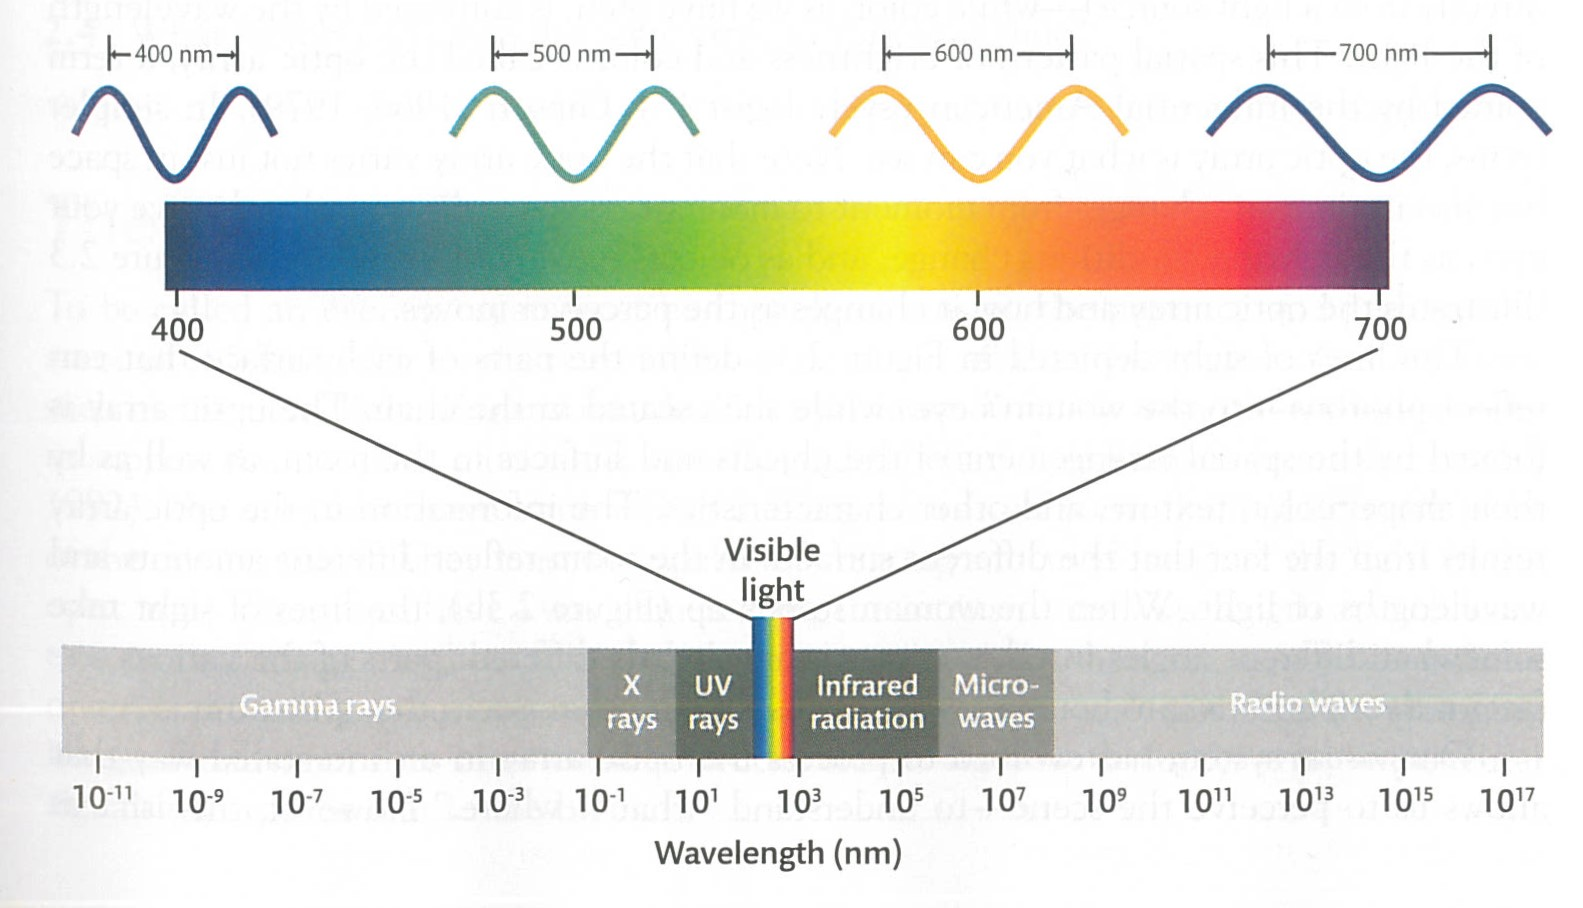
\includegraphics[width=0.8\textwidth]{img/EMSpectrum.jpg}
  \caption{The electromagnetic spectrum\goodcite{hsp}}
  \label{fig:EMSpectrum}
\end{figure}
Even though this explanation is adequate for the physical aspect, there is still different theories on how exactly we will perceive the colours in the spectrum. But for this comparison we will only be covering the photoreceptors and how they function.% But it is still evident that the cones in an eye is sensitive to respective wavelengths.\\

%\subsubsection{Trichromatic \& Opponent-process theory} %
%\label{sec:colour-trichro-n-dichro}
%One evident theory is the Trichromacy theory, which explains that there's three types of cones, each sensitive to their respective wavelength. This is a result of the photosensitive pigment in each of the cones, being sensitive to different wavelengths\goodcite{hsp}.\medskip \\

%The opponent-process theory, explains how we typically perceive colours to be off of 4 basic colours; these being: Yellow, Green, Red, Blue\goodcite{hsp}. The reason for this is brain circuits interpreting the receptive signals, and example is the adaptation.

\subsubsection{The human eye \& Photoreceptors}
Simply, light enters the eye through the Cornea, which then further travels through the Lens past the Iris, through the Vitreous chamber and finally arrives at the Fovea, where the light is focused to form an image of the currently viewed scene.\goodcite{hsp}.\\The Lens and Cornea helps to focus the image and the Iris helps to determine how much light should be let in through the rest of the eye. To focus the image, the Lens functions to refract the incoming light, to make sure the light is properly focused when it reaches the retina\goodcite{hsp}.\medskip \\

\begin{figure}[H]
    \centering
    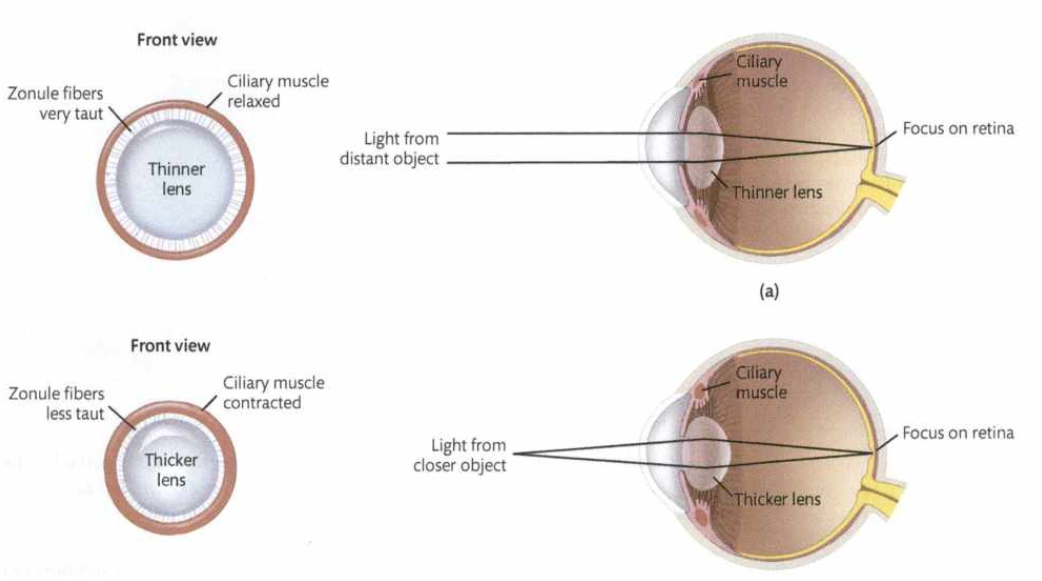
\includegraphics[width=\textwidth]{img/eyelens.png}
    \caption{Focusing light in the eye\goodcite{hsp}}
    \label{fig:focus_light}
\end{figure}

Adjusting the shape of a lens, the focal point can be altered and thereby determining the position of where the lightrays should focus. The Lens in the eye will be stretched by muscles, to focus on objects that are at different distances in a scene, see \autoref{fig:focus_light}. This specific adjustment in the lens and eye is called \texttt{accomodation}\goodcite{hsp}.\medskip\\

%\subsubsection{Photoreceptors}
The photoreceptors in the eyes' retina consists of rods and cones, which are two types of neurons which transduce light into neural signals. The cones carry the information of the difference in wavelength. The cones are also sensitive to different wavelengths, namely short, medium and long wavelengths, whereas the rods do not carry much information in regards to wavelength, but are much more sensitive to the intensity of light\goodcite{hsp}.\\After the light has been converted into neural signals, they get propagated through multiple other cells and finally to the retinal ganglion cells, which axons bundle together and send action potentials(AP) to the brain, thereby enabling the brain to perceive colour.\goodcite{hsp}.\\

\subsubsection{Cameras \& Digital sensors}
Similar to the lens in an eye, the lens of a camera aim to duplicate the functionalities for getting a sharp and clear image\goodcite{IP}. More specifically, the lens is an important factor in optical systems, which serves to focus incoming light, typically onto a set of sensors\goodcite{IP}. Another aspect is also how the aperture in a camera, resembles the iris functionalities, controlling how much light should be allowed to pass through. A camera with a low shutter speed of the aperture can potentially result in blurry images if too much movement is in the scene while the image is captured\goodcite{IP}. This is although not the case with the human eyes' iris, as it just serves to not overwhelm the rods and cones with light\goodcite{hsp}.

\begin{figure}[H]
    \centering
    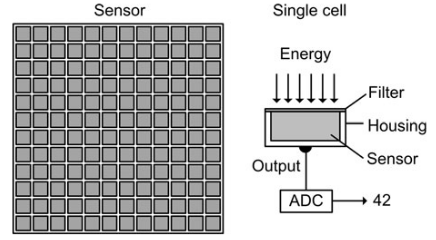
\includegraphics[width=0.8\textwidth]{img/sensor.png}
    \caption{Image sensor\goodcite{IP}}
    \label{fig:Image_sensor}
\end{figure}

A likely candidate for the cones in an eye, and how they function, would be the sensor in a digital camera. The digital sensor is a grid of interconnected cells, respectively the red, green and blue have filters for allowing certain energy to enter the cells, this is stored as voltage which will be converted to a digital number through a converter\goodcite{IP}. This method of storing electromagnetic waves as energy, resembles how the rods and cones in the retina store the electromagnetic waves, and more specifically the sensitivity to the respective wavelengths\goodcite{hsp}.\\The digital sensor will then convert the retrieved wave energy into digital numbers, typically in a three-dimensional vector that represents the RGB color-space\goodcite{IP}. This resembles how the retina also transduce light into colour and intensity, by the rods and cones, which are sent further to the brain by the propagated information from the cells in the retina.\goodcite{hsp}.

%%%%%%%%%%%%%%%%%%%%%%%%%%
%%%%% Next Topic %%%%%%%%%
%%%%%%%%%%%%%%%%%%%%%%%%%%

\subsection{Recognizing visual objects}% w * 2
This section will cover the comparisons of the Gestalt principles of figure ground organization and edge completion, compared to BLOB analysis and thresholding.\medskip\\

Recognizing objects might be a simple task for a human, but it shows to be a lot more than just visually perceiving an object. Multiple elements play a role in proper object recognition, such as Figure-Ground organization, Perceptual grouping, Perceptual interpolation, recognition by components model, edge detection and the Gestalt principles\goodcite{hsp}.\\
%\begin{figure}
%    \centering
%    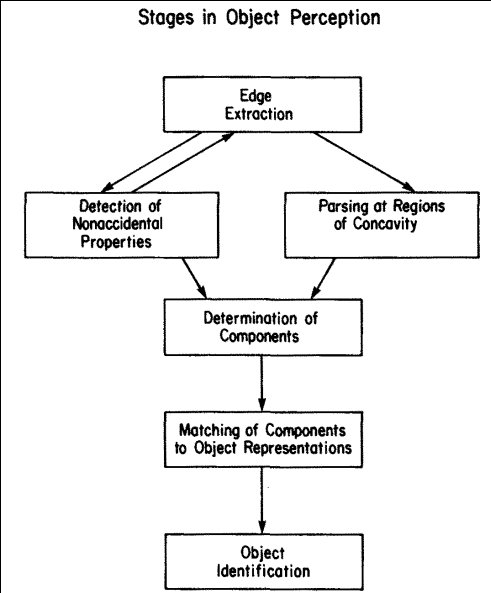
\includegraphics[width=0.5\textwidth]{img/ObjectSteps.png}
%    \caption{Stuff}
%    \label{fig:ObjectHiarchy}
%\end{figure}
The steps for recognizing visual objects is split into two layers, firstly the perceptual organization which generally includes the pattern of neural activity to represent edges and regions, dividing these regions and grouping them with similar properties whilst at the end filling in missing elements. The second layer being the object recognition, which matches the candidate objects to the representations stored in memory\goodcite{hsp}\goodcite{bieder}.

\subsubsection{Figure Ground Organization}
\label{sec:perceptialorganization}
Perceptual organization serves to make object recognition in complex scenes possible, it does this by performing a certain amount of steps to candidate objects in the scene, for later recognition\goodcite{hsp}.\\
Three complications are quite important, when talking about the analysis of object recognition, these three are called the following; image clutter, object variety and variable views.\\
Image clutter refers to the fact that multiple objects in a scene may occlude each other, where the visual system must make up for the occluded parts of objects. The object variety refers to how many different objects there is it generally recognize, this is in terms of shape and form. Even if the object is difficult to specifically identify, a general idea of what the object is can still be found. Variable views, is how an object can appear differently on the retinal images, depending on the orientation and the viewpoint of the object whilst also being of different illumination\goodcite{hsp}.\\

% THIS CAN BE RELATED TO THE SEMESTER PROJECT IN TERMS OF HAND EDGES AND REGION(BLOB ANALYSIS & EDGE DETECTION(CONVEX HULL))
The edges and regions of a figure, are "detected" by patterns of neural activity, responding to location, orientation and curvature of objects in a simple scene, a scene with only contrast in intensity. This process is performed by the visual system and is called \textit{edge extraction}. This can be more abstract when reviewing an image of more complex intensity of brightness, an example could be any scene with occlusion, shadows or shading on an object which also refers to the previously used term; image clutter. The question then becomes, how can the brain then resolve the complex or cluttered scenes?\\
% blabla image processing

% MORE ABOUT HSP
This question can be answered by covering multiple topics which makes up good candidates for the second layer of recognizing visual objects. The Gestalt psychology gives an overview of how different principles can give better meaning to a scene\goodcite{hsp}. For example dividing the regions into figure and ground, to explain this simply, it is the identification of a figure from a background. The figure and ground organization is only one of multiple perceptual grouping techniques used to identify figures in a scene. The reasoning for the identification in terms of Gestalt psychology, is that the figure or region, is typically perceived as such because it is surrounded by another region.\\Logically, this must mean that the figure is occluding the background.\goodcite{hsp}\\

\begin{figure}[H]
    \centering
    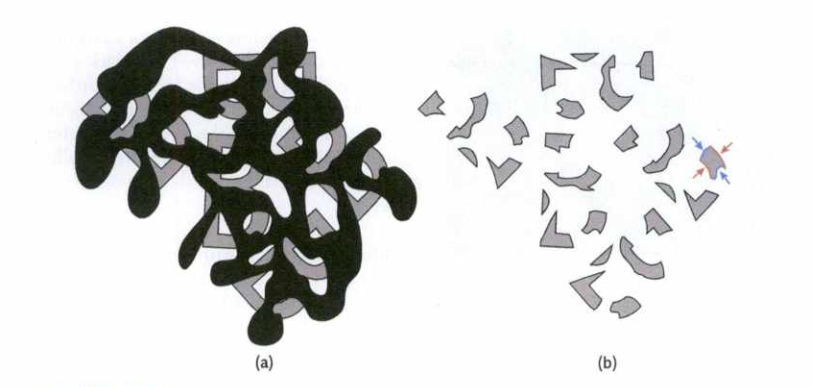
\includegraphics[width=\textwidth]{img/b.png}
    \caption{Illustration of Border Ownership and Figure-ground Organization\goodcite{hsp}}
    \label{fig:border_ownership}
\end{figure}

\autoref{fig:border_ownership} illustrates the grouping technique of border ownership and figure-ground organization, on the left figure (a) it is easier to determine the borders and therefore easier to determine the occluded letters B. Whereas on the right figure (b), it is harder since the visual system gives all the fragment borders ownership (Which makes them seem like individual figures)\goodcite{hsp}.\medskip \\Another example is edge completion, which sets up illusory contours which perceptually fill in missing edges to complete figures. An example would be three circles which all have a small triangle shape cut out of them all, but the circles are aligned to certain angles to give off the illusion that there is a triangle to be perceived in the missing space, between the circles.\\
\subsubsection{BLOB Analysis}
A likely media-technological relative to the figure-ground organization could be BLOB(Binary Large OBject) analysis, which is a technique in Image Processing. BLOB analysis is the extraction of features and classification of a BLOB, in an image\goodcite{IP}. The BLOB will then be classified as an arbitrary object in the image\goodcite{IP}.\\It does this by going through each individual pixel in an image, and then classifying the different pixels according to their neighbours, the classification of which pixels belong to what classified object is determined by the kernel used in the process.\goodcite{IP}.\medskip \\

Referring to the \autoref{fig:border_ownership} again, the BLOB analysis would to a certain extent, also arrive at the same result as the average human would perceive. Since the right figure (b), where the fragments have no interconnection, the BLOB analysis would regard all the fragments as individual BLOBs, whereas the right figure (a) would be determined as one whole (keeping in mind that the ink would have to be the same colour as the occluded letters). BLOB classification would also potentially classify the ink as one object, the fragments as multiple single objects, whereas the Gestalt psychology suggest that edge completion supports that the perceived letters behind the ink are perceived as whole objects, in this case the whole letter B. Keep in mind that this only applies to very simple scenes, whereas if BLOB analysis was used directly on a complex or cluttered scene, it would definitely fail. Therefore a big difference is that BLOB analysis does require multiple other libraries or algorithms to do its job properly.\medskip\\

Another candidate for a related media-technological counterpart to the figure-ground organization, more specifically detecting edges from intensity of colour and/or luminosity, could be Thresholding. Thresholding is the process of mapping a certain range of pixels with a specific pixel-value to either 0 or 255, or 0 and 1\goodcite{IP}. Thresholding takes a specific thresholding value, which it then compares to all the pixels of an image. If the pixel-value is lower than the threshold value then it assigns the pixel-value to 0 whilst the reverse operation is applied to pixel-values above the threshold value\goodcite{IP}.\\This will help segment figures that are of different colour and/or luminosity from the rest of the image clutter.\medskip \\

One potentially huge difference here is the processing power, for doing BLOB classification or extraction a whole image needs to be read, whereas there is no requirement laid out that the visual system needs to operate on every little detail in a scene and can potentially through top-down information, decide how much and what information is important enough to process.

%%%%%%%%%%%%%%%%%%%%%%%%%%
%%%%% Next Topic %%%%%%%%%
%%%%%%%%%%%%%%%%%%%%%%%%%%

\subsection{Object recognition}
This section will compare the resemblance of object recognition, against a likely media-technological counterpart called Feature matching or potentially template matching.
\subsubsection{Object recognition}
After the creation of candidate objects by the perceptual organization steps, the visual system now has to recognize the objects. This is done by matching the objects, to stored memory in the brain.\\

It makes sense to claim that the visual system must somehow be able to compare objects to memory, despite changes in viewpoints of said object. A visual system that can achieve this, exhibits \textit{invariance}\goodcite{hsp}.\\There are different approaches to how invariance is achieved by the visual system, one of them being the recognition by components model. This model is built on how object recognition depends on; \textit{"identifying the primitive geometrical components that make up the object"}\goodcite{hsp}.\\This is illustrated on \autoref{fig:components}, by looking at figure (c) and figure (d), it is clear how the location of the handle denotes whether the object is a cup or that of a bucket.

\begin{figure}[H]
    \centering
    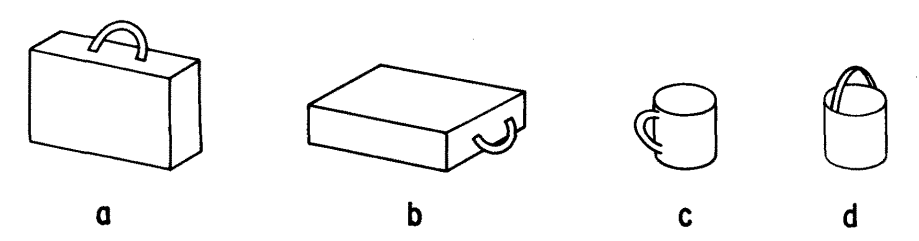
\includegraphics[width=\textwidth]{img/comps.png}
    \caption{Different arrangement of components produce different objects.\goodcite{bieder}}
    \label{fig:components}
\end{figure}

Another approach to invariance, is that it is based on a view-specific manner, in which multiple representations of a single object would be stored. Multiple different views of a single object will be stored, and when the current view will give off a specific view of an object, all the stored views will be compared simultaneously, enabling the brain to recognize the object from differing viewpoints.\medskip \\

\subsubsection{Feature matching}
Computer-vision specific techniques that exhibit part wise the same traits as the view-specific manner of approaching invariance, is the feature matching approach in computer-vision.\\Feature matching takes certain features of an object and matches it against objects in a scene and retrieves the most likely match based on distance calculations\goodcite{OpenCV}, see \autoref{fig:feature_matching} for an illustration of how feature matching functions with a scene and a template image.\medskip \\

\begin{figure}[H]
    \centering
    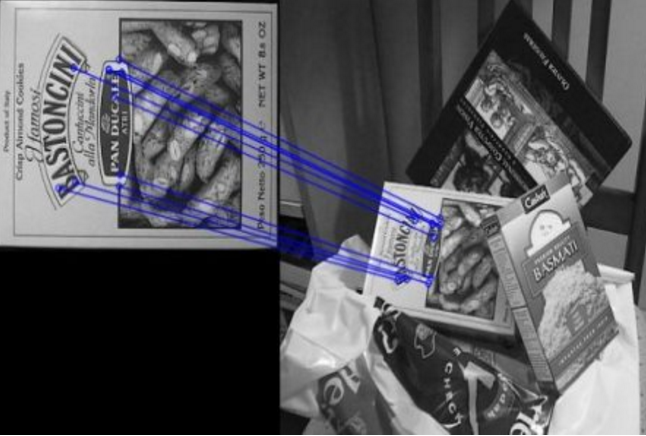
\includegraphics[width=0.7\textwidth]{img/featurematch.png}
    \caption{Feature matching in OpenCV\goodcite{OpenCV}}
    \label{fig:feature_matching}
\end{figure}

%The task of finding correspondences between two images of the same scene or
%object is part of many computer vision applications. Camera calibration, 3D
%reconstruction, image registration, and object recognition are just a few. The
%search for discrete image correspondences – the goal of this work – can be di-
%vided into three main steps. First, ‘interest points’ are selected at distinctive
%locations in the image, such as corners, blobs, and T-junctions. The most valu-
%able property of an interest point detector is its repeatability, i.e. whether it
%reliably finds the same interest points under different viewing conditions. Next,
%the neighbourhood of every interest point is represented by a feature vector. This
%descriptor has to be distinctive and, at the same time, robust to noise, detec-
%tion errors, and geometric and photometric deformations. Finally, the descriptor
%vectors are matched between different images. The matching is often based on a
%distance between the vectors, e.g. the Mahalanobis or Euclidean distance. The
%dimension of the descriptor has a direct impact on the time this takes, and a
%lower number of dimensions is therefore desirable.
%It has been our goal to develop both a detector

Keeping in mind that we still have insufficient knowledge on how exactly object recognition occurs, but by utilising and constructing artificial systems, based on our visual system and the theories of how we perceive the world, a potential explanation of how it functions could be presented\goodcite{solveVisual}.\\
The authors of \texttt{How Does the Brain Solve Visual Object Recognition?} claim that the techniques can be explored by applying the theoretical aspect as algorithms in the artificial system, thereby a synergy between the relevant research fields which look at the artificial system in correlation to how perceptual system functions, could be a solution for understanding object recognition\goodcite{solveVisual}.\\
\begin{center}
    \textit{"We expect this pace to accelerate, to fully explain human abilities, to reveal ways for extending and generalizing beyond those abilities, and to expose ways to repair broken neuronal circuits and augment normal circuits."}\goodcite{solveVisual}\medskip \\
\end{center}
Many of the techniques explained in this essay are only potential counterparts, but it can help us explore how our own brain functions in regards to the media-technological topics. A big difference is that computers are accessing data sequentially, whereas the brain can do it near instantly with simultaneous firing neurons..
% Medialogy related problems. Give at least three examples of technological advancements, where knowledge of human perception has been (or would be crucial) for the technological advances. How was the innovation

% Comments about object recognition theories
% Invariance, constancy, two theories(suggestions) critics on second theory
% First theory very abstract
% - We store generalized small objects and depending on the combination of the simple objects, we form a greater object to recognize, this is also affected by the viewpoint
% -
% Second theory
% - We store all information about an object, how we match it depends on the similarity of the images, e.g. 3 angles of a car are very similar = same object.

%\section{Summarization}
% Color & Eye vs Camera & Digital Sensors
% BLOB & Thresholding vs Perceptual Organization
% Feature matching vs Object Recognition
\newpage
\section{Bibliography}
\label{sec:Bibliography}
\printbibliography

\end{document}
